
\documentclass[10 pt,usenames,dvipsnames, oneside]{article}
\usepackage{../../modelo-fracoes}
\graphicspath{{../../../Figuras/licao03/}}


\begin{document}

\begin{center}
  \begin{minipage}[l]{3cm}
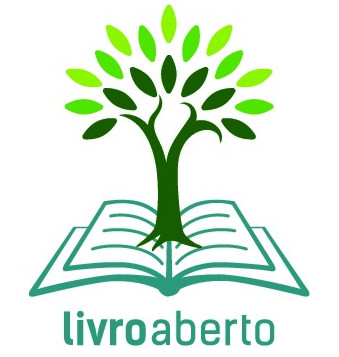
\includegraphics[width=2cm]{../../../Figuras/logo}       
\end{minipage}\hfill
\begin{minipage}[r]{.8\textwidth}
 {\Large \scshape Atividade: Mapa do tesouro}  
\end{minipage}
\end{center}
\vspace{.2cm}

\ifdefined\prof
%Caixa do Para o Professor
\begin{goals}
%Objetivos específicos
\begin{enumerate}
\item Marcar frações na reta numérica.
\item Comparar frações com o mesmo numerador.
\end{enumerate}

\tcblower

%Orientações e sugestões
\begin{itemize}
\item Observe que, nesta atividade, a unidade não está destacada na reta a partir dos pontos 0 e 1, como nas atividades anteriores. Oriente seu aluno a identificar o zero como o ponto correspondente à palmeira imperial.
\item Esclareça aos seus alunos que o caminho todo, da palmeira à pedra, não é a unidade. Peça-os que estimem quantas unidades tem esse caminho.
\item Reproduza a faixa que indica a unidade e distribua uma para cada estudante. Oriente-os a dobrá-la para resolver o item a).
\item Observe que o aluno pode responder o item b), comparando as frações $\frac{5}{6}$ e $\frac{5}{8}$, sem considerar a marcação feita no item a). De fato, como $\frac{1}{6} > \frac{1}{8}$, sabe-se que $\frac{5}{6} > \frac{5}{8}$ e, portanto, o tesouro está no baú que está a $\frac{5}{6}$ da unidade da palmeira.
Explore essa discussão com a turma.
\end{itemize}
\end{goals}

\bigskip
\begin{center}
{\large \scshape Atividade}
\end{center}
\fi

Um caçador de tesouros encontrou o mapa e o papiro a seguir. Leia as instruções para a localização do tesouro e decida em que local ele deve cavar.

\begin{figure}[H]
\centering

\begin{tikzpicture}[x=1cm,y=1cm, every node/.style={scale=1.10}, scale=1.10]

\node (mapa) at (3,2) {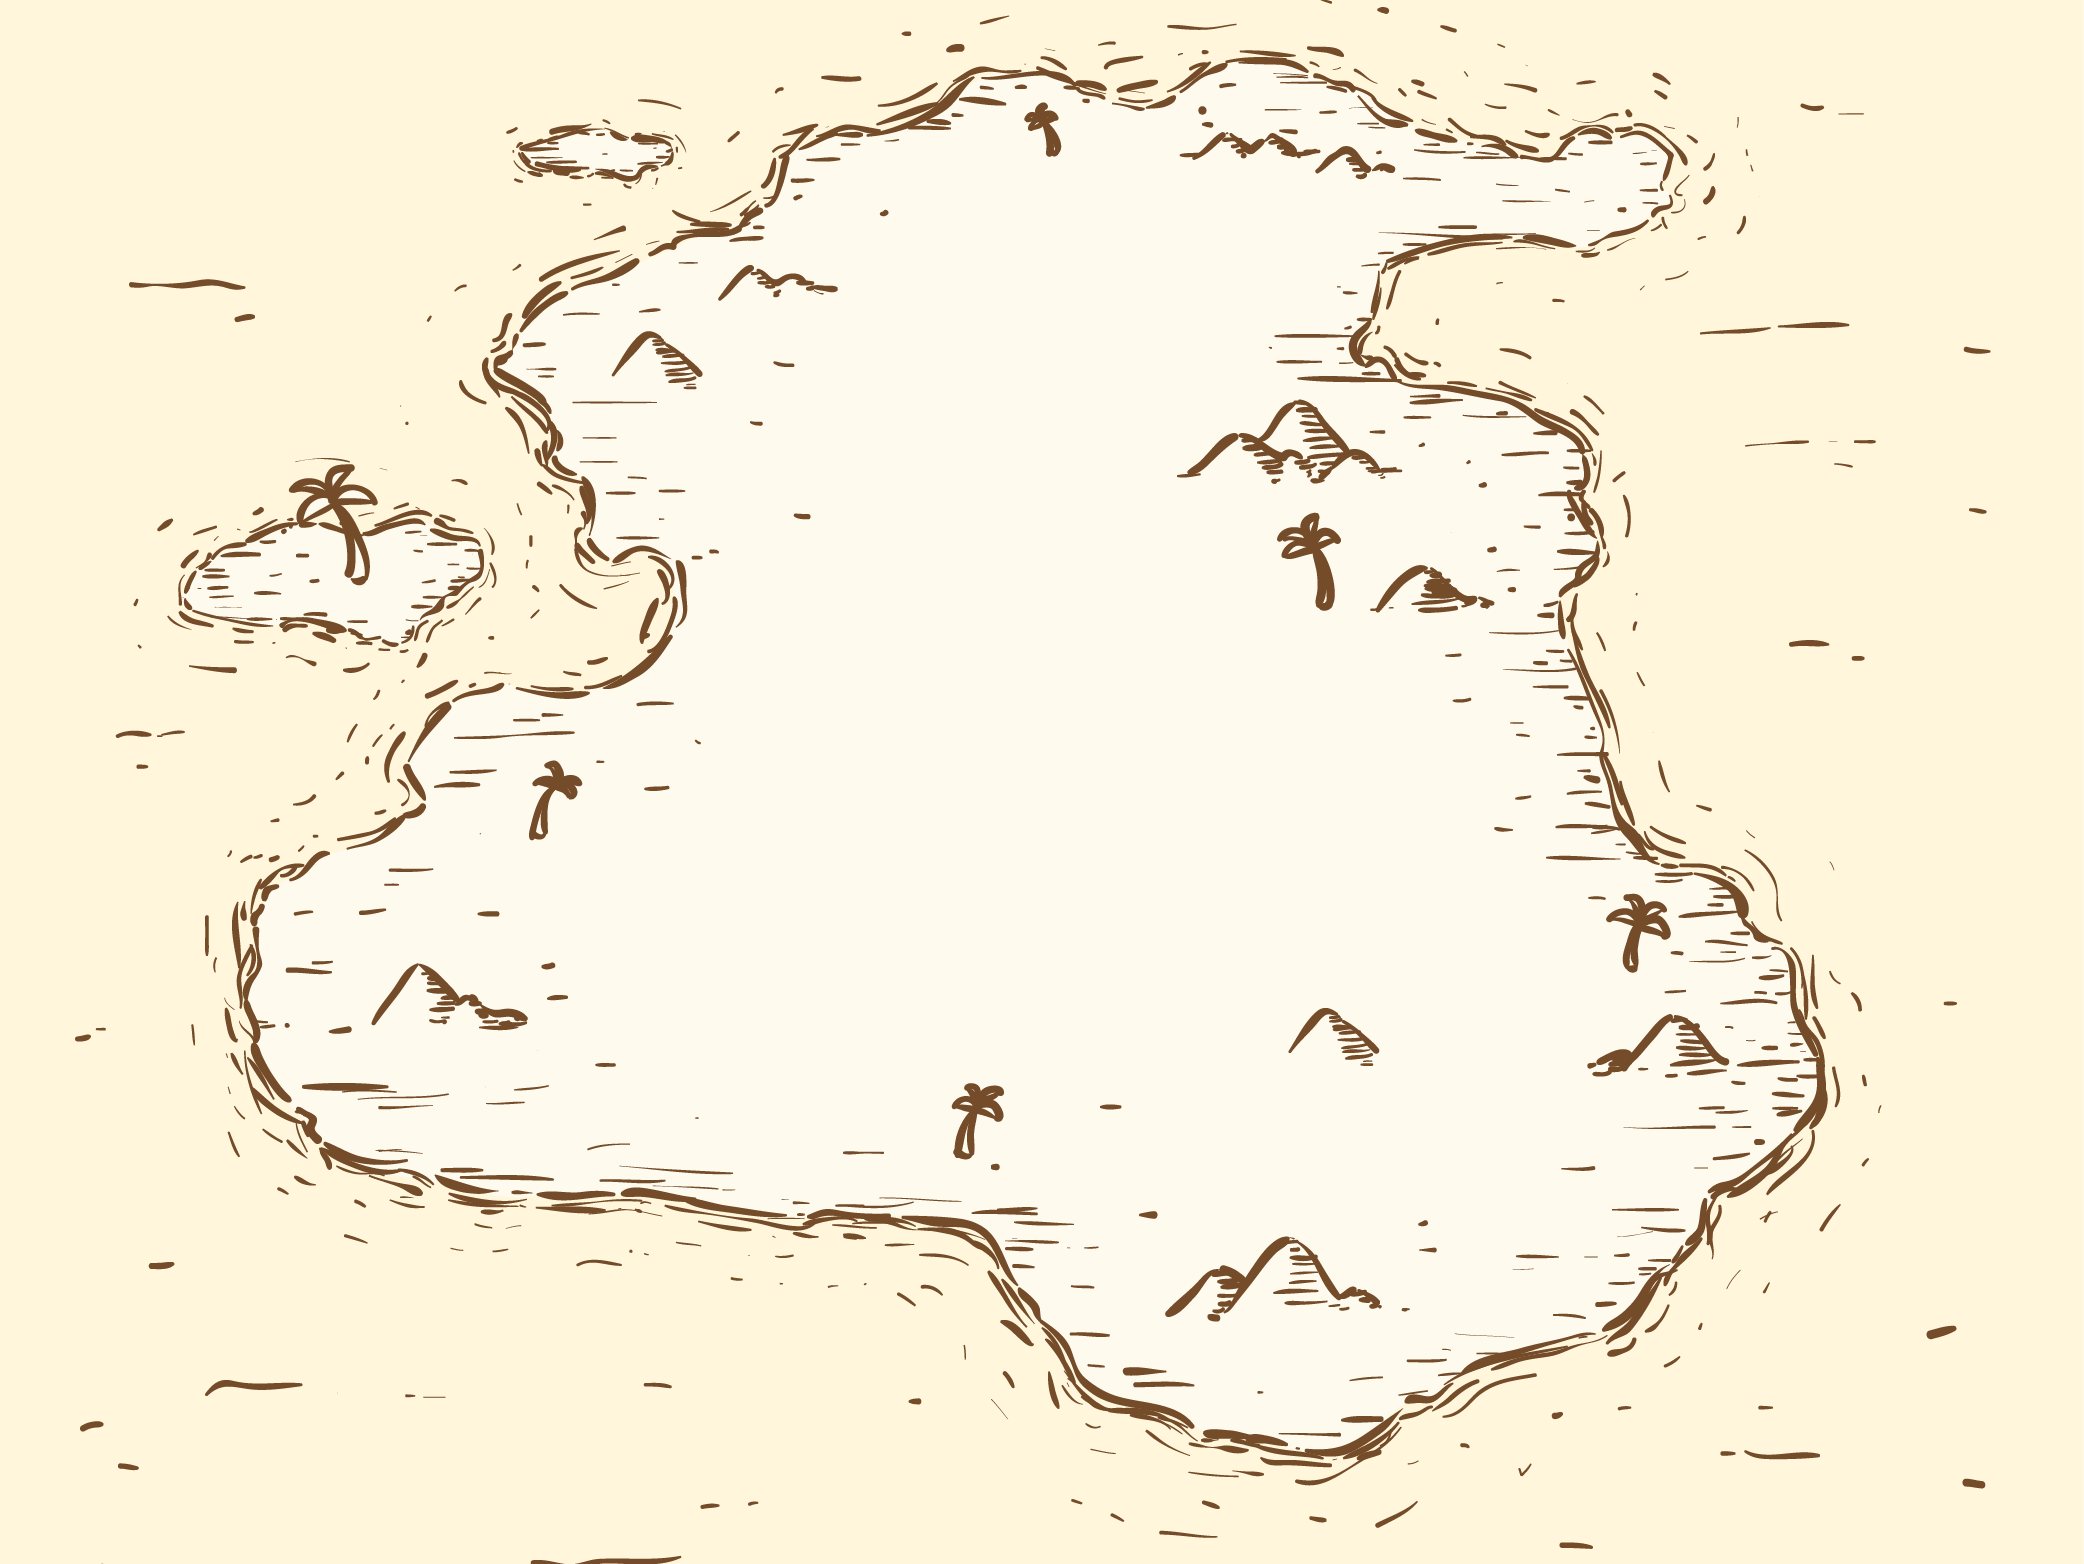
\includegraphics[width=300bp]{mapa.png}};
\node at (.8,0.65) (palm) {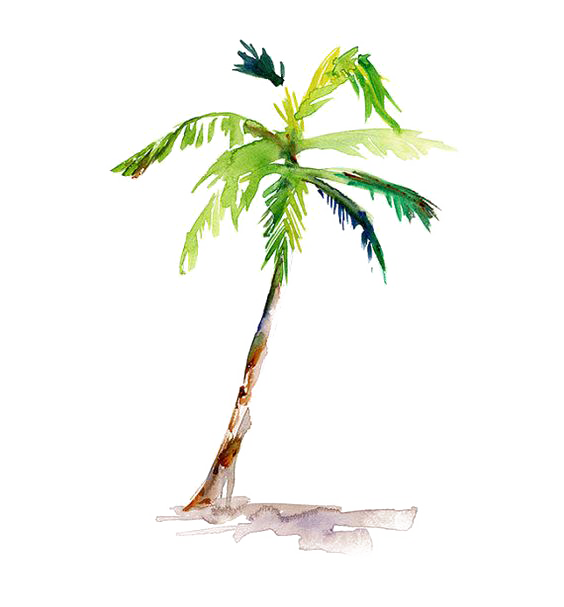
\includegraphics[width=50bp]{palmeira.png}};

\node (pedra) at (4.28,3.85) {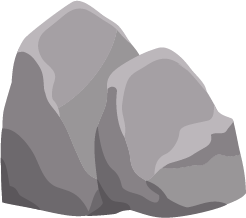
\includegraphics[width=33bp]{pedra.png}};

\draw [dashed] (.85,.1) -- (3.9,3.3);

\draw [ultra thick, red] (3,2) -- (4.5,2);
\end{tikzpicture}

\begin{tikzpicture}
\setlength{\baselineskip}{15pt}
\setlength\parskip{.1em}
\node [scale=0.9] {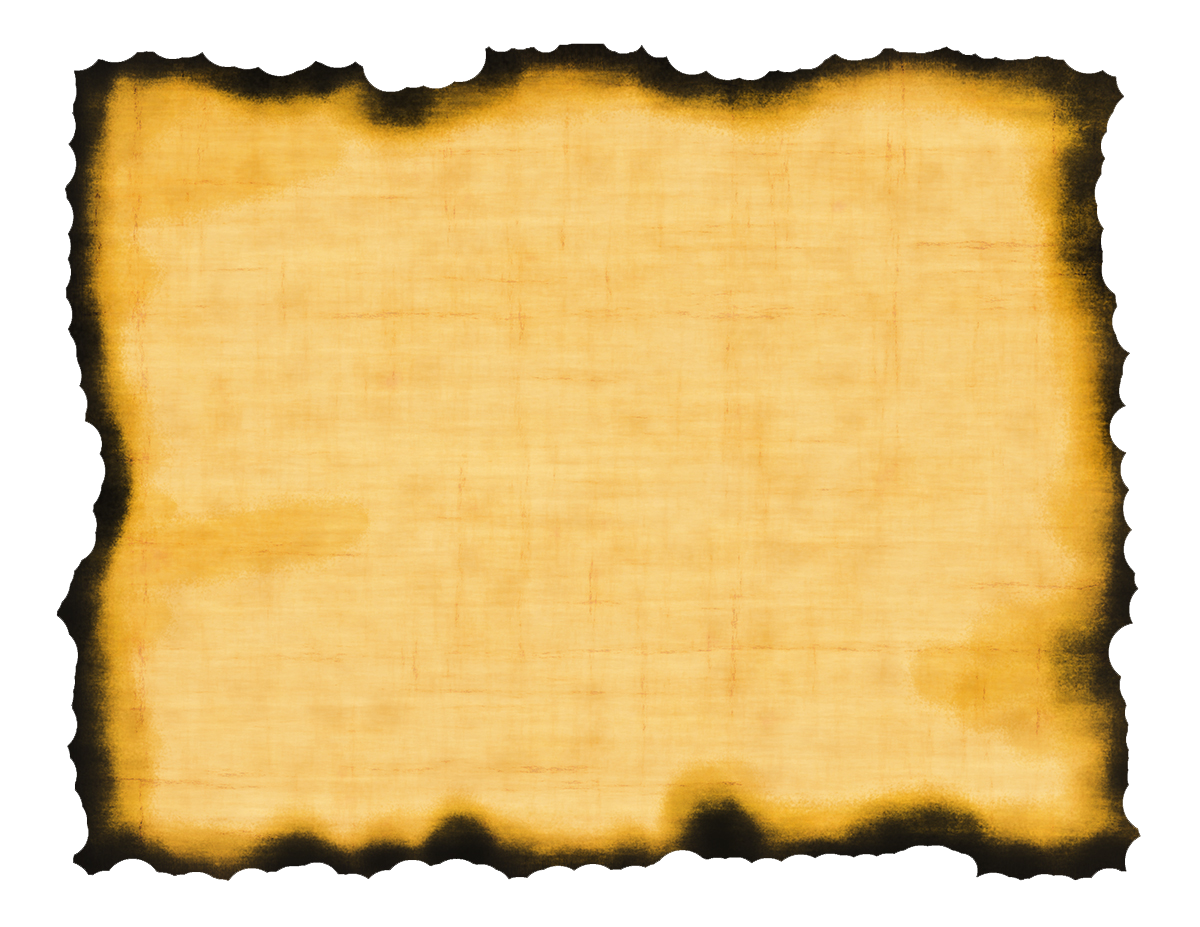
\includegraphics[width=410bp]{papiro.png}};
\node [rectangle]{\parbox{275bp}{
Há dois baús escondidos, um deles carregado com um tesouro. Para localizá-los, você deve seguir o mapa e estas instruções.


\begin{enumerate}[label=\arabic*.,topsep=.5em]
\setlength{\baselineskip}{15pt}
\setlength\parskip{.1em}

\item Use a faixa vermelha como unidade para descobrir a localização dos baús.
\item Os baús estão enterrados no caminho em destaque, alinhados com a palmeira imperial e com a pedra.
\item No mapa, os pontos que marcam os locais em que os baús estão enterrados ficam a $\frac{5}{6}$ e a $\frac{5}{8}$ da unidade, a partir da palmeira. A chave do baú com o tesouro está enterrada a $\frac{13}{8}$ da unidade a partir da palmeira.
\item O baú com o tesouro está mais distante da palmeira.

\end{enumerate}}};
\end{tikzpicture}
\end{figure}

% \noindent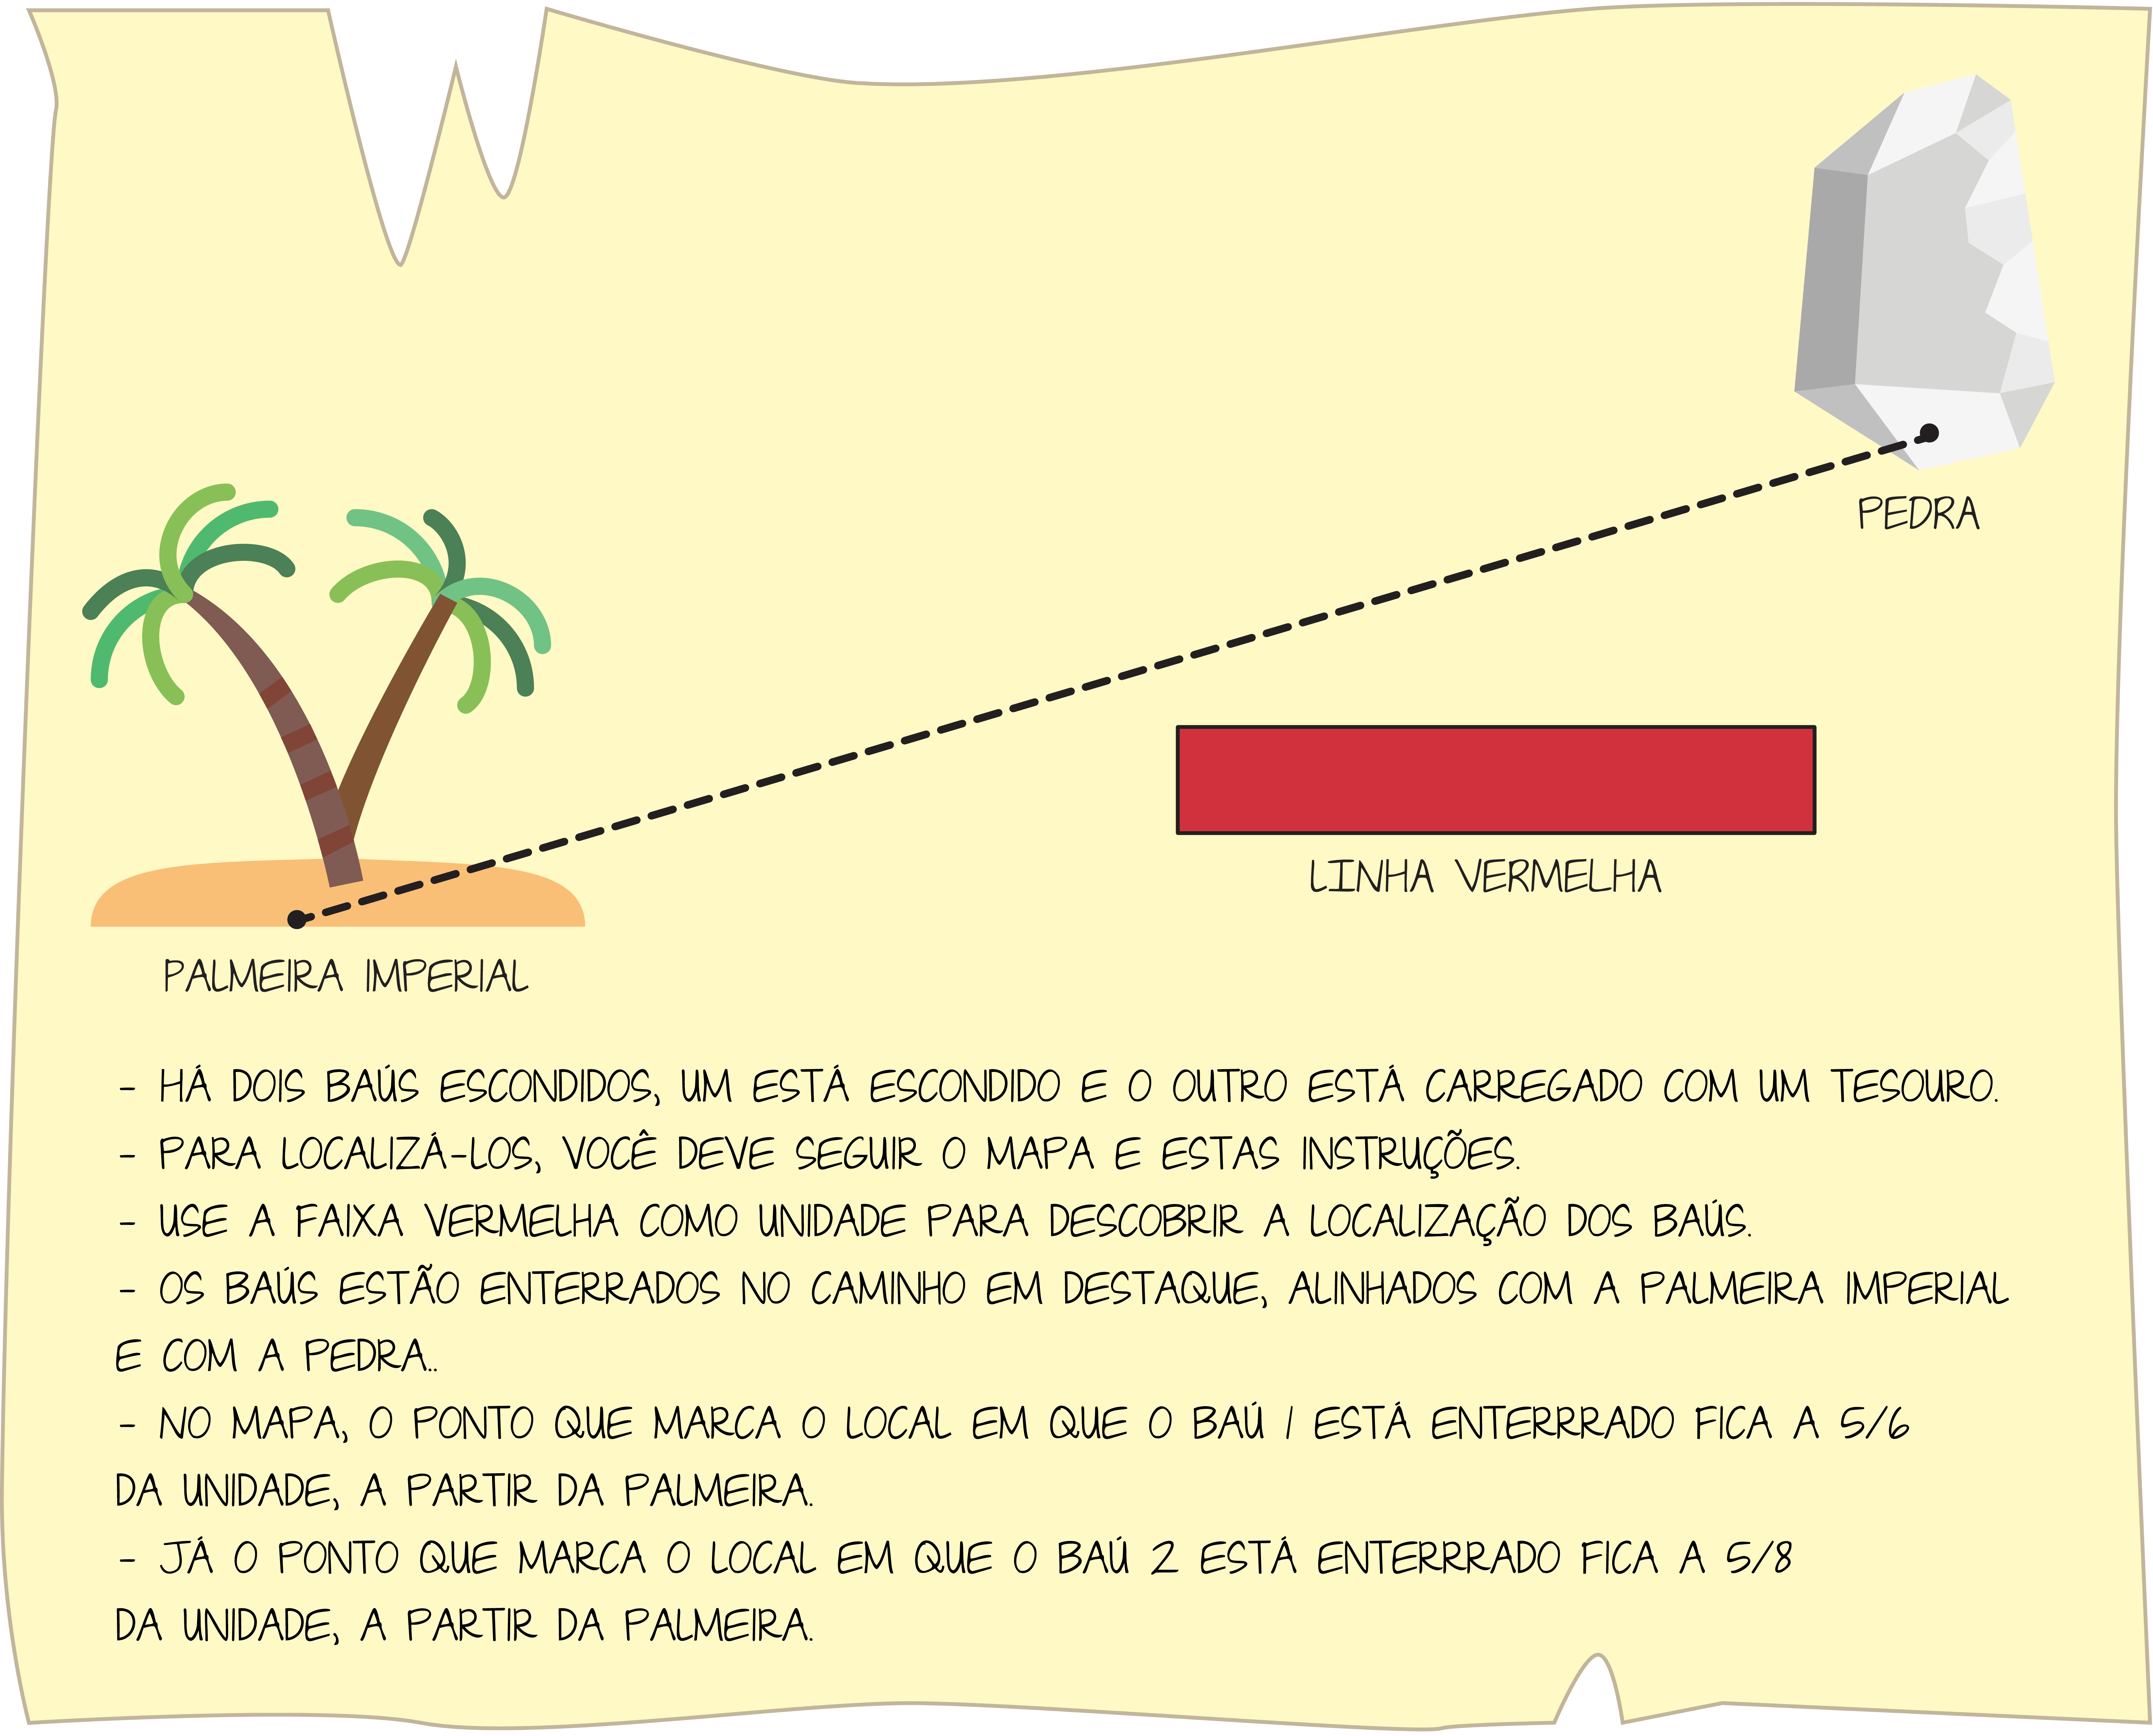
\includegraphics[width=\textwidth, keepaspectratio]{../figuras/licao03/ativ7_fig01.png}

\begin{enumerate}
 \item Marque, no mapa, as localizações dos baús e da chave.
 \item Qual o baú com o tesouro? Explique como chegou à sua conclusão.
\end{enumerate}

\ifdefined\prof
\begin{solucao}

 \begin{enumerate}
 \item
 \adjustbox{valign=t}
 {
  \begin{tikzpicture}[scale=.5, x=1cm, y=1cm, every node/.style={scale=1.25}]
   \filldraw[fill=attention, opacity=.3] (0,-.5) rectangle (10,.5);
   \draw[dashed] (0,0) -- (18,0);
   \node[below] at (10,-.3) {1};
   \filldraw[fill=common] (0,0) circle (.3);
   \node[above] at (0,.3) {Palmeira};
   \node[below] at (0,-.3) {0};
   %\fill[common] (16,0) circle (.3);
   %\node[above] at (16,0) {Pedra};
   \filldraw[fill=attention] (6.25,0) circle (.3);
   \node[above right, rotate=30] at (6.25,.3) {Baú};
   \node[below] at (6.25,-.3) {$\frac{5}{8}$};
   \filldraw[fill=attention] (8.33,0) circle (.3);
   \node[above right, rotate=30] at (8.33,.3) {Baú};
   \node[below] at (8.33,-.3) {$\frac{5}{6}$};
   \filldraw[fill=attention] (16.25,0) circle (.3);
   \node[above] at (16.25,0) {Chave};
   \node[below] at (16.25,-.3) {$\frac{13}{8}$};
  \end{tikzpicture}
 }
  \item  O baú com o tesouro é o que está a $\frac{5}{6}$ da unidade da palmeira, uma vez que $\frac{5}{6} > \frac{5}{8}$. 
\end{enumerate}

\end{solucao}
\fi

\end{document}